\documentclass[conference]{IEEEtran}
\usepackage{amsmath,amssymb,amsfonts}
\usepackage{algorithmic}
\usepackage{graphicx}
\usepackage{textcomp}
\usepackage{xcolor}
\usepackage{biblatex}
\usepackage{titlesec}
\usepackage{float}
\usepackage{listings,xcolor}



\def\BibTeX{{\rm B\kern-.05em{\sc i\kern-.025em b}\kern-.08em
		T\kern-.1667em\lower.7ex\hbox{E}\kern-.125emX}}


\addbibresource{references.bib}

\begin{document}

	
\title{Speaker Voice Similarity Analysis and Evaluation}

	
\author{\IEEEauthorblockN{Carmel Gafa}
	\date{April 2025}
	
}

\maketitle

\begin{abstract}
This study investigates the effectiveness of a WavLM-based system in distinguishing between 285 different speakers from the ABI-1 dataset. \end{abstract}



\section{Introduction}

Speaker identification is the determination of a speaker's identity from a segment of their speech. It is crucial in applications such as personalized voice assistants, security systems, and partitioning audio streams according to each speaker's identity. Unlike speech recognition, which focuses on what is being said, speaker identification is concerned with who is speaking.

This task can effectively be approached as a downstream application of pre-trained self-supervised speech models, such as \texttt{Wav2Vec2}\cite{baevski2020wav2vec} or its enhanced variant \texttt{WavLM}\cite{chen2022wavlm}. These models are trained on large-scale unlabelled audio datasets to learn audio representations that capture phonetic and speaker-specific characteristics.

In this project, \texttt{WavLM-base-plus-sv}, a fine-tuned version of \texttt{WavLM} specialized for speaker verification, is used to extract speaker embeddings from audio samples. These embeddings are compared using cosine similarity to measure the similarity of two voice samples. This architecture enables a simple speaker identification pipeline without the need to train a model from scratch.


\section{Data preprocessing}
\label{sec:data-processing}

The Accents of the British Isles (ABI) Corpus represents 13 regional accents. Figure \ref{fig:img-abi-corpus-accents} shows how these accents are categorized into four broad accent groups; Scottish, Irish, Northern English, and Southern English. Each broad group is further split into its respective regional accents\cite{najafian2016improving}.

\begin{figure}[H]
	\centering
	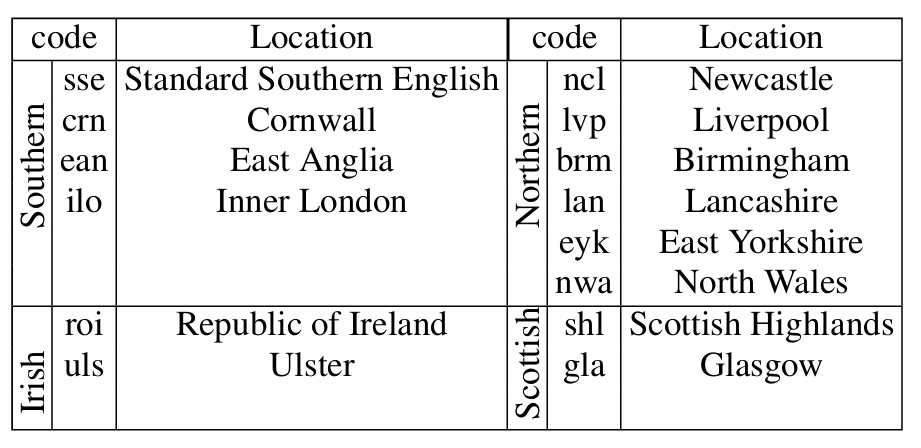
\includegraphics[width=0.7\linewidth]{img/img-abi-corpus-accents}
	\caption{List of accent codes and their corresponding geographical locations in the ABI-1 corpus\cite{najafian2016improving}. The accents are grouped into four regional categories: Southern, Irish, Northern, and Scottish. This structure is used throughout the analysis to evaluate speaker similarity across and within regional accent groups.}
	\label{fig:img-abi-corpus-accents}
\end{figure}

The corpus includes 285 subjects, with speech collected from individuals who have lived in each regional accent area since birth. Each of the 285 subjects read the same three short passages. These are short paragraphs forming the 'sailor passage', with lengths of 92, 92, and 107 words with average durations of 43.2, 48.1, and 53.4 seconds, respectively\cite{najafian2016improving}.

The sources do not explicitly describe the recording conditions of the ABI corpus, however, it is mentioned that the speakers were selected by a phonetician, suggesting an effort for a standard quality recording for at least that accent\cite{najafian2016improving}.

\subsection{Signal resampling}
\label{ssec:signal-resampling}

Audio signals depend on two main parameters

\begin{itemize}
	\item number of channels $C$, that is $1$ for mono and $2$ for stereo.
	\item number of samples $T = t \times f_s$; that in turn depends on the
	\begin{itemize}
		\item duration $t$ of the audio in seconds.
		\item sampling rate $f_s$ (e.g. 48,000 Hz).
	\end{itemize}
	
\end{itemize}

For a mono signal, that is common in these applications, a vector representing the utterance is available for processing,  $\mathbf{x}_{\text{raw}} \in \mathbb{R}^{1 \times T}$ in this way.


The model by Microsoft that we are using in this example expects a signal rate of 16,000 Hz, and it is therefore necessary to resample the signal to this frequency. The resampling step involves selecting a subset of samples from the original vector, so that the original sampling rate $f_s^{\text{raw}}$ becomes a lower one $f_s^{\text{target}}$. The down-sampling ratio in this case, $R = \frac{f_s^{\text{raw}}}{f_s^{\text{target}}} = 3$


Before reducing the number of samples, the high-frequency components from the original signals are removed, as they could cause aliasing. Aliasing occurs when frequencies above the new Nyquist frequency (which is one-half the new sampling rate) “fold back” into the signal, corrupting it. The Nyquist frequency after down-sampling becomes:

$$f_N^{\text{new}} = \frac{f_s^{\text{target}}}{2} = 8000~\text{Hz}$$

To remove the high frequency components, a low-pass filter is applied, generating a filtered signal, $\tilde{x}$

$$\tilde{x}[n] = x_{raw}[n] * h[n]$$

where $h[n]$ is the impulse response of a low-pass filter, typically a windowed \texttt{sinc} function:

$$h[n] = \text{sinc}\left(\frac{n}{R}\right) \cdot w[n]$$

Here, $w[n]$ is a window function (like Kaiser, Hamming, etc.) to localize the infinite \texttt{sinc} filter in time.

If, as an example, we consider this function:

\begin{align*}
	x_{raw} &=[x[0], x[1], x[2], x[3], x[4], x[5], x[6], x[7], x[8]]\\
		 	&=[2, 4, 6, 8, 10, 8, 6, 4, 2]
\end{align*}

and use the following windowed \texttt{sinc} filter (kernel)

\begin{align*}
	h &= [h[0],\ h[1],\ h[2]]\\
	  &= [0.2,\ 0.6,\ 0.2]
\end{align*}

We slide the kernel over the signal and compute:

$$\tilde{x}[n] = \sum_{k=0}^{2} x[n + k] \cdot h[k]$$

So that the first two samples of the filtered signal becomes

\begin{align*}
	\tilde{x}[0]	&= 0.2 \cdot x[0] + 0.6 \cdot x[1] + 0.2 \cdot x[2] \\
					&= 0.2\cdot2 + 0.6\cdot4 + 0.2\cdot6 \\
					&= 0.4 + 2.4 + 1.2 \\
					&= 4.0\\
	\tilde{x}[1] 	&= 0.2 \cdot x[1] + 0.6 \cdot x[2] + 0.2 \cdot x[3] \\
					&= 0.2\cdot4 + 0.6\cdot6 + 0.2\cdot8 \\
					&= 0.8 + 3.6 + 1.6 \\
					&= 6.0
\end{align*}

Once the signal is filtered, we can keep every $R^\text{th}$ sample and discard the rest (decimation), or alternatively, apply interpolation to produce a smoother, resampled signal at the desired rate.

$$x_{\downarrow R}[n] = x[Rn]$$

So that, for example,

$$x_{\downarrow 3}[n] = x[0], x[3], x[6], x[9], \dots$$


\begin{figure}[H]
	\centering
	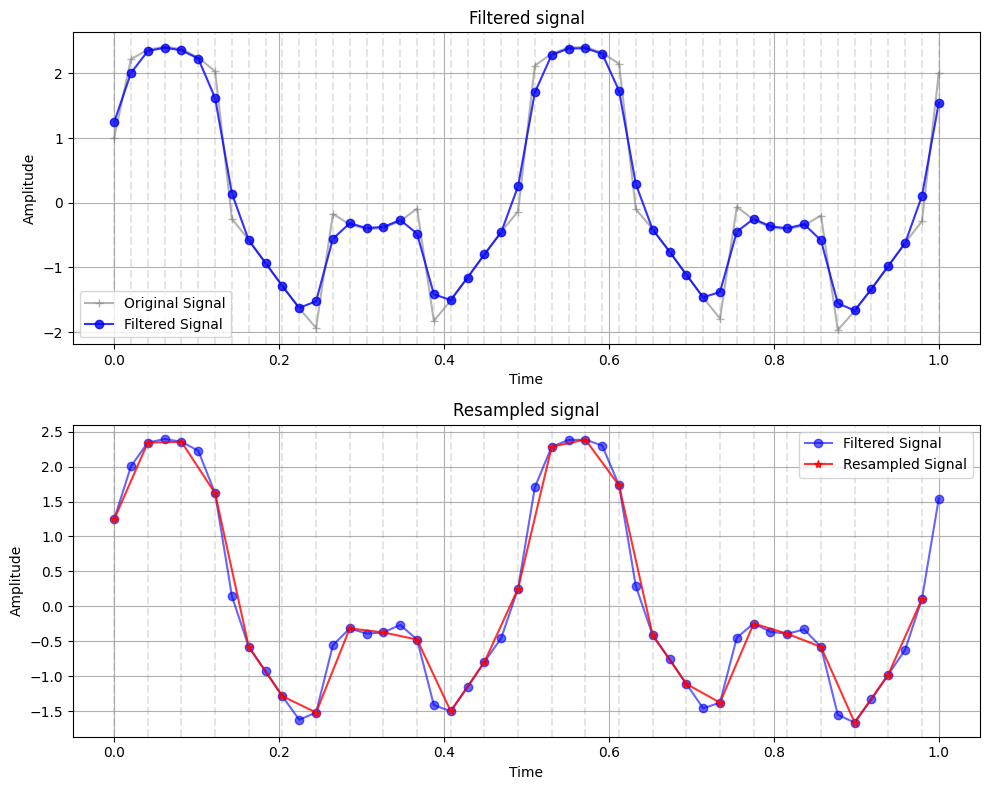
\includegraphics[width=0.9\linewidth]{img/img-resampling}
	\caption{Visualization of the signal processing steps applied during audio preprocessing. The top plot shows the original and filtered signals, highlighting the smoothing effect of the filter. The bottom plot illustrates the effect of resampling the filtered signal to a target rate (e.g., 16\,kHz), with the resampled signal closely tracking the filtered one, preserving the original signal’s structure while adjusting its temporal resolution.}
	\label{fig:img-resampling}
\end{figure}




\section{Methodology}

In this section, we will discuss the implementation of the speaker voice similarity comparison pipeline. Several general criteria were observed during this exercise:
\begin{itemize}
	\item Code that manipulated data was implemented in Python scripts, whereas code that analysed data in Python notebooks. This approach is preferred for several reasons:
	\begin{itemize}
		\item Scripts encourage modularity better.
		\item It is easier to import developed functions when using scripts.
		\item Scripts avoid the notebook's overheads like kernel restarts and variable state issues.
		\item The notebooks' interactive nature makes them very attractive for data analysis and tasks with a predominant visualisation component.
	\end{itemize}
	\item The analysis of voice similarity is broken down into discrete steps and implemented as stand-alone modules.    Each module will generate one or more results that are, in most cases, based on the results generated by previous modules in the pipeline. This approach is inspired from the medallion architecture that is widely used in industry.
	\item Modules are stringed logically together to perform all the tasks necessary in this project, including the download of the data and model.
	\item Data is manipulated only using code. The whole project can be executed without any manual intervention whatsoever.
	\item Wherever possible, an option to execute the appropriate parts of a module on the GPU was made available.
	\item A simple logging tool was created so all modules can inject information about their execution. This logger is also used by a timer decorator that was created to measure the duration of the various modules of this project.
\end{itemize}

\subsection{Comparison strategy}
\label{ssec:comparison-strategy}

As discussed in Section \ref{sec:data-processing}, three audio files are available for each speaker in the ABI-1 dataset, and these will be used to determine the similarity of any speaker to all other speakers in the dataset. The following approach is used to determine similarity in this exercise.

Each audio file is compared with the other audio files for a given speaker, a total of $\binom{3}{2} = 3$ comparisons, and the minimum value is retained as the intra-comparison result.

For every speaker combination in the dataset, each audio file of one speaker is compared to all the audio files of the other speaker, a total of nine comparisons and the maxim value is retained as the inter-comparison result.

This approach will determine the thresholds and results that ensure maximum separation, as the minimum distance between intra and inter-comparisons will be examined.



\subsection{Voice similarity comparison pipeline}

\begin{figure}[H]
	\centering
	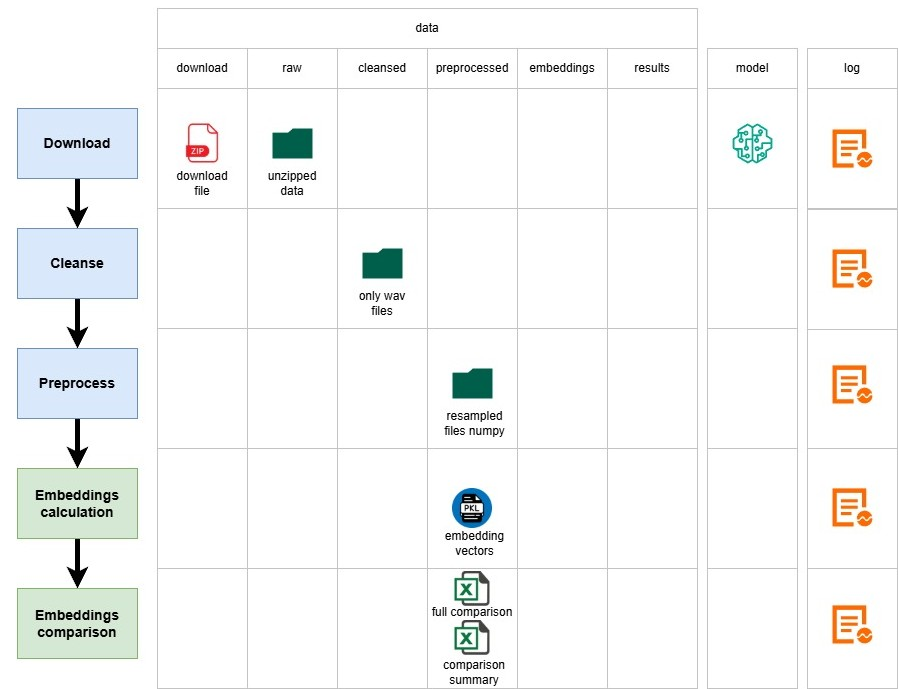
\includegraphics[width=1\linewidth]{img/img-pipeline}
	\caption{Overview of the speaker similarity analysis pipeline and associated file structure. Each processing stage—download, cleanse, preprocess, embeddings calculation, and embeddings comparison—produces outputs stored in dedicated folders. The flow diagram on the left outlines the logical sequence, while the table maps each module to its corresponding outputs across the \texttt{data}, \texttt{model}, and \texttt{log} directories.}
	
	\label{fig:img-pipeline}
\end{figure}

Figure \ref{fig:img-pipeline} shows the flow that was implemented as part of this project, which is made up of the following modules:
\begin{itemize}
	\item \textbf{Download}. In the first step of the pipeline, the \texttt{ABI-1} dataset archive is downloaded and placed in the \texttt{data/download} folder. The contents are then extracted and placed in the \texttt{data/raw folder}. The \texttt{ABI-1} structure has an \texttt{accents/genders/speakers} structure, whereby accents folders contain a male and female folder for each speaker. At this point, the data also contains additional data, such as transcription information.
	The \texttt{wavlm-base-plus-sv} model is also downloaded from Hugging Face using the \texttt{transformers} library and placed in the \texttt{model} folder.
	This module also contains the functionality to create the data, module and log folder structure that is necessary for this project.
	
	\item \textbf{Cleanse}. In the next step, the contents of each speaker, in each gender and each accent in the raw data are examined, and the files matching the pattern \texttt{shortpassage*.wav} are retained. The results are placed in an identical folder structure in the \texttt{data/cleansed} folder.
	
	\item \textbf{Preprocess}. As we have discussed in Section \ref{ssec:signal-resampling}, the audio files need are preprocessed to 16KHz using \texttt{torchaudio.transforms.Resample} so that their embeddings can be evaluated by the model. In this next step, all the audio files of each speaker, in each gender and accent in the raw data folder are loaded and resampled. The resulting \texttt{numpy} arrays are placed in an identical folder structure in \texttt{data/preprocessed}.
	
	\item \textbf{Embedding calculation}. In the next step, the \texttt{wavlm-base-plus-sv} model calculates the embeddings for each audio data file. Each embedding is effectively a 512-element vector, so a $3 \times 512$ array is created for each speaker. The embedding information was stored in a dictionary data structure with "\texttt{accent-gender-speaker}" as key and the embedding array as the value during processing. It was then converted to a \texttt{pandas} \texttt{DataFrame} and saved as a pickle file in the \texttt{data/embeddings}.
	
	\item \textbf{Comparison}. The final step of the pipeline implements pairwise cosine-similarity using the strategy explained in Section \ref{ssec:comparison-strategy}. Two files are generated in this process:
	\begin{itemize}
		\item A raw results file contains the results of all comparisons: a set of three for intra-comparison and a set of nine for inter-comparison.
		\item A summary results file that contains the selected comparison from each set using the strategy described previously.
	\end{itemize}
	The result files are stored in the \texttt{data/results} folder
\end{itemize}

\section{Evaluation and results}

The analysis presented in this section was conducted using the \texttt{analysis.ipynb} Jupyter notebook to evaluate the performance of the WavLM model in a speaker similarity context. 
This notebook serves as an important component of the evaluation pipeline, delivering insight into the separability of speaker embeddings and the robustness of the overall system.

Figure~\ref{fig:img-self-similarity} presents a histogram showing the distribution of cosine similarity values obtained from intra-speaker comparisons.

As described in Section~\ref{ssec:comparison-strategy}, each value in this plot represents the minimum similarity between two utterances from the same speaker.

We can see that most of the same-speaker similarity scores fall within a high similarity range between approximately 0.985 and 0.997. 

\begin{figure}[H]
	\centering
	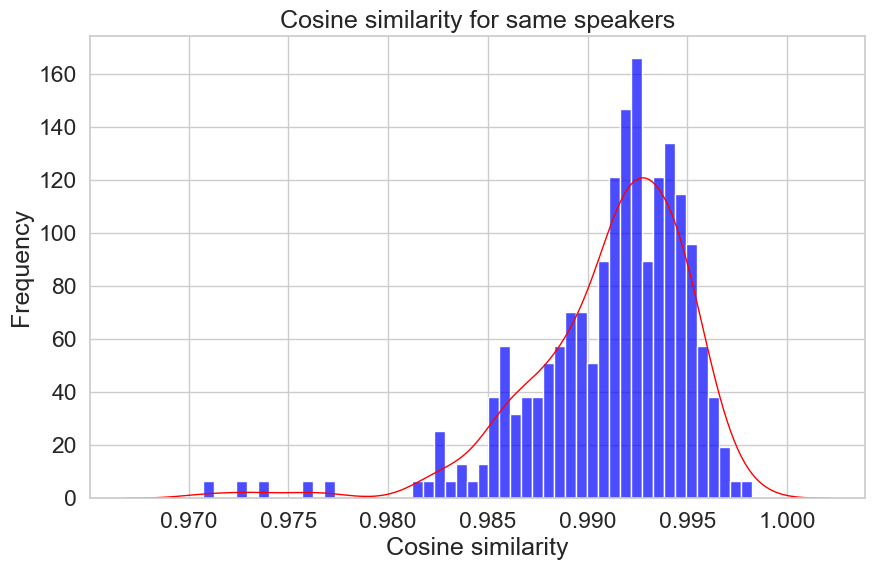
\includegraphics[width=0.7\linewidth]{img/img-self-similarity}
	\caption{Distribution of cosine similarity scores for same-speaker comparisons. The histogram shows a strong concentration of similarity values in the 0.985–0.997 range, indicating high consistency of embeddings produced by the WavLM model for recordings from the same speaker. A slight leftward tail suggests occasional variability due to acoustic or recording conditions.}
	\label{fig:img-self-similarity}
\end{figure}


As expected, these results are tightly concentrated around the upper bound of the cosine similarity scale, showing that the WavLM model produces highly consistent embeddings for recordings belonging to the same speaker. 

The distribution also shows a small leftward tail, with a few similarity values extending up to 0.970. These lower outliers could be attributed to several factors, including acoustic variability across recordings, differences in speaking style or vocal effort, or background noise. We are saving the minimum intra-similarity metric and maintaining all low-scoring outliers without offsetting them with possibly better values.

Nevertheless, the number of such occurrences is small relative to the full dataset, and the core of the distribution remains strongly peaked at higher similarity values.

Overall, this analysis confirms the robustness and discriminative power of the speaker embeddings generated by WavLM for intra-speaker comparison tasks, which is both expected and highly desirable. This result can form a solid foundation upon which reliable threshold-based decisions can be made.


Figure~\ref{fig:img-similarity} displays the distribution of cosine similarity scores computed between speakers of different genders. Each score represents the maximum similarity between utterances from two distinct male and female speakers.

Unlike the tightly clustered same-speaker distribution shown in Figure~\ref{fig:img-self-similarity}, this distribution is broader and centred significantly lower on the cosine similarity scale. Most values fall between 0.55 and 0.85, with a peak around 0.72. This spread is expected, as embeddings from different speakers—particularly those differing in vocal pitch and timbre due to gender—are naturally more dissimilar.

\begin{figure}[H]
	\centering
	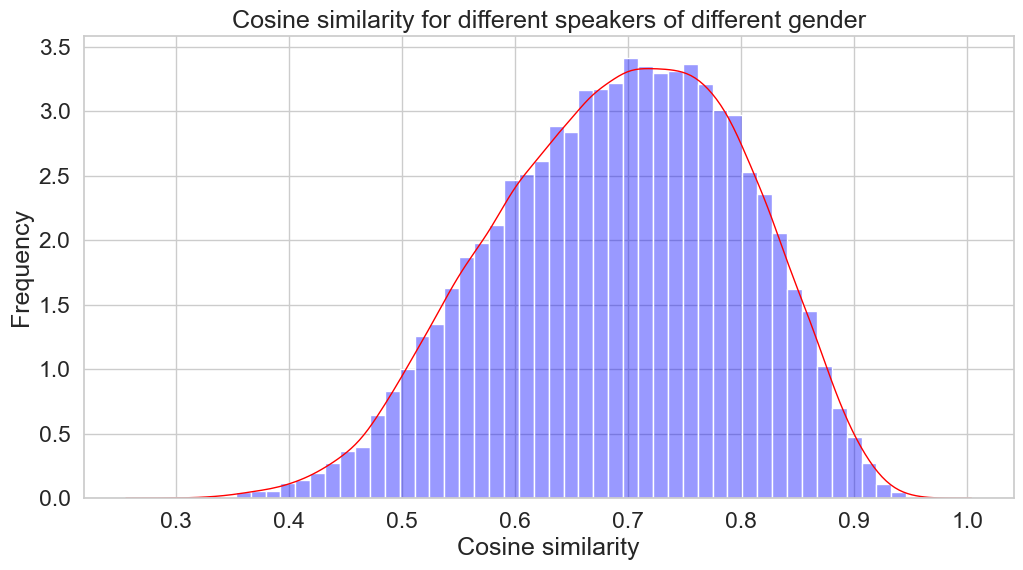
\includegraphics[width=0.7\linewidth]{img/img-similarity}
	\caption{Distribution of cosine similarity scores for different-speaker comparisons across genders. The histogram shows a wider and lower-centered distribution relative to same-speaker similarities, with the majority of values ranging between 0.55 and 0.85.}
	\label{fig:img-similarity}
\end{figure}


The model demonstrates a good separation between same-speaker and cross-gender different-speaker comparisons. The minimal overlap between the lower tail of same-speaker scores observed in Figure~\ref{fig:img-self-similarity} and the upper tail of this distribution provides a practical rationale for selecting a threshold that effectively discriminates between same and different speakers.

\begin{figure}[H]
	\centering
	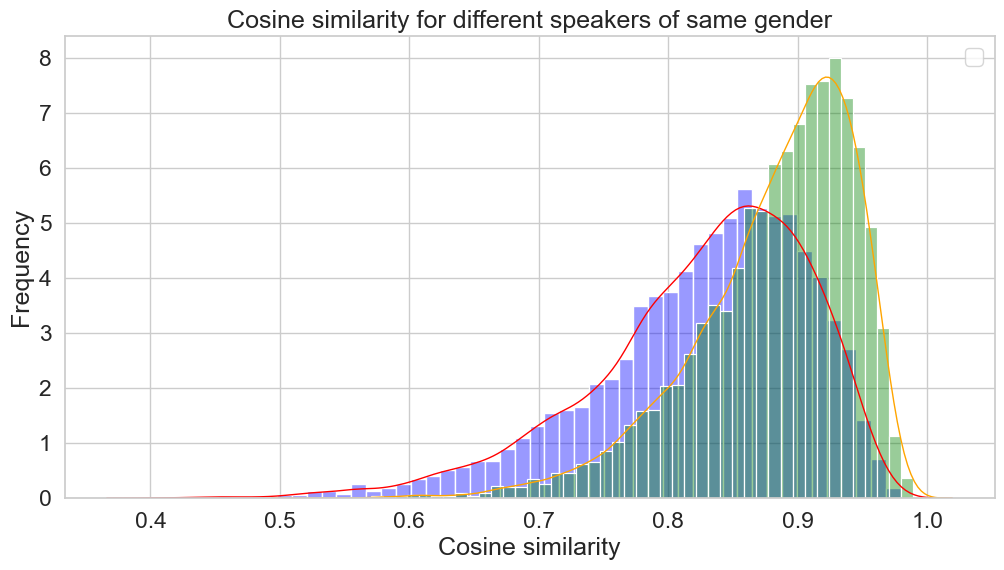
\includegraphics[width=0.7\linewidth]{img/img-similarity-same-gender}
	\caption{Distribution of cosine similarity scores for different-speaker comparisons within the same gender. The histogram distinguishes between male-male (blue) and female-female (green) speaker pairs. Both distributions exhibit higher similarity values compared to cross-gender comparisons, with substantial overlap and peaks in the range of 0.85 to 0.95.}	
	\label{fig:img-similarity-same-gender}
\end{figure}

Figure~\ref{fig:img-similarity-same-gender} illustrates the distribution of cosine similarity scores computed between speakers of the same gender, separated into male-male and female-female speaker pairings. Each value corresponds to the maximum similarity score observed among all utterance pairs between two distinct speakers within the same gender category.

In contrast to the cross-gender distribution shown in Figure~\ref{fig:img-similarity}, male and female same-gender distributions are noticeably skewed toward higher similarity values. Most scores lie between 0.80 and 0.97, with both curves peaking at approximately 0.88 to 0.92. This increased similarity is likely due to shared vocal characteristics such as pitch range, speaking style, and formant patterns that are more common within the same gender group.

While these distributions are distinguishable from same-speaker comparisons of Figure~\ref{fig:img-self-similarity}, they exhibit greater overlap with the same-speaker tail, particularly in the upper similarity range, presenting a more challenging case for threshold selection, as overly conservative thresholds may begin misclassifying some different-speaker pairs as same-speaker matches.

\begin{figure}[H]
	\centering
	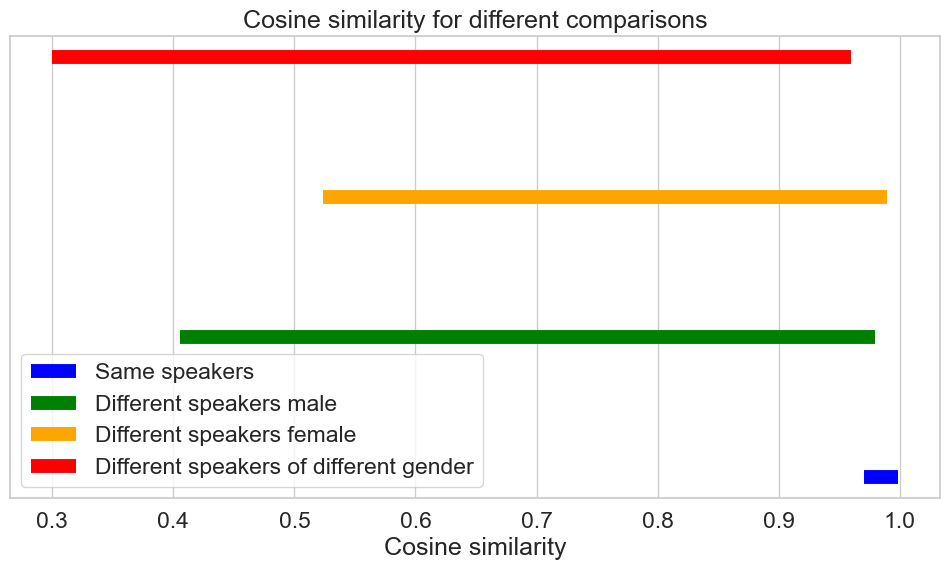
\includegraphics[width=0.7\linewidth]{img/img-similarity-comparison}
	\caption{Cosine similarity ranges across speaker comparison categories. Each horizontal bar represents the observed similarity range for a particular group: same-speaker pairs (blue), different speakers of the same gender (green and orange), and different speakers of different genders (red). This visual summary highlights the separation between intra- and inter-speaker similarities, supporting the choice of an effective threshold for speaker verification.}
	\label{fig:img-similarity-comparison}
\end{figure}

Figure~\ref{fig:img-similarity-comparison} summarises the cosine similarity ranges observed across all comparison categories analysed in the previous figures. Each horizontal bar illustrates the full range of similarity scores for a specific comparison group: same-speaker, male-male, female-female, and cross-gender pairs.

The same-speaker scores form a narrow, high-range band, with values consistently close to 1.0. In contrast, all inter-speaker groups span broader ranges and are centred at lower similarity values. Cross-gender comparisons occupy the lowest band, typically ranging from 0.30 to 0.95, while same-gender comparisons show higher overlap with the same-speaker band, peaking near 0.90 or slightly above.

This summary illustrates that while some overlap exists between same-speaker and same-gender different-speaker comparisons, especially near the upper ends of the distributions, there remains a significant gap that allows for a robust decision threshold definition.

A well-chosen threshold, in the 0.95–0.98 range, can effectively separate same-speaker matches from different-speaker mismatches while minimising false acceptances and rejections.

\subsection{Threshold selection}

In the previous section, we noticed that the number of different-speaker pairs vastly exceeds that of same-speaker pairs, resulting in an insignificant imbalance in the dataset.

In this case, traditional metrics such as accuracy can be misleading as a model biased toward predicting "different "speakers can still achieve high accuracy without performing well on identifying same-speaker pairs. 

F1 score provides a more informative measure in this context,  as it captures the harmonic mean of precision and recall, thereby balancing the trade-off between false positives and false negatives. As we will see in this section, the F1 score remains low for most thresholds but exhibits a sharp peak at a specific value, indicating a precise point at which the model achieves its best balance of sensitivity and specificity. 


\begin{figure}[H]
	\centering
	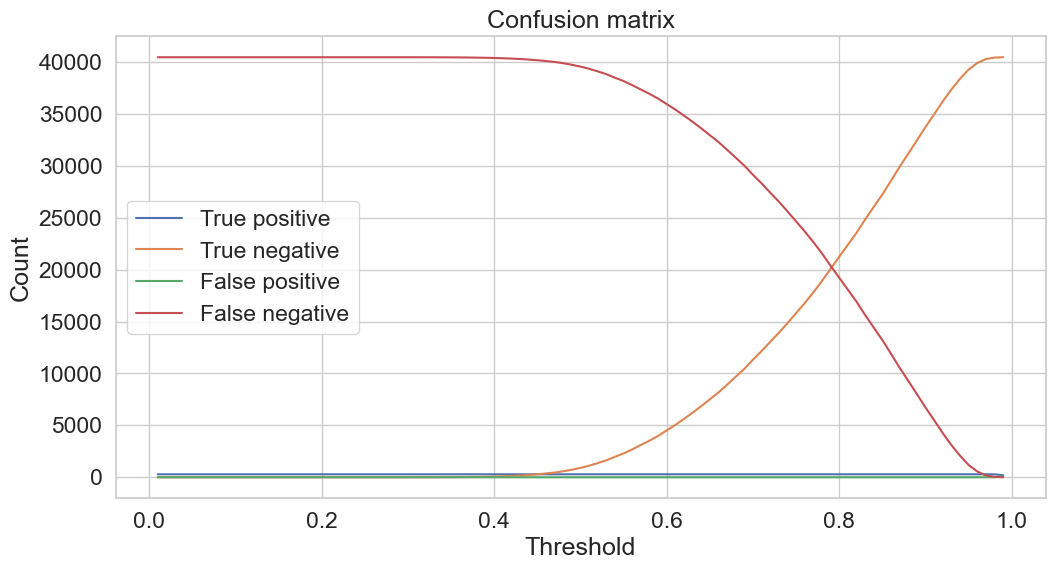
\includegraphics[width=0.7\linewidth]{img/img-confusion-matrix}
	\caption{Variation of confusion matrix components as a function of the similarity threshold. The plot shows how true positives, true negatives, false positives, and false negatives evolve as the decision boundary is adjusted. This visualisation aids in selecting a threshold that balances correct classification and error rates for speaker verification.}
	\label{fig:img-confusion-matrix}
\end{figure}


Figure~\ref{fig:img-confusion-matrix} illustrates how the components of the confusion matrix evolve as a function of the decision threshold applied to cosine similarity scores.

This plot was generated using a threshold sweep and classifying speaker pairs as same-speaker if their similarity exceeds the current threshold.


\begin{figure}[H]
	\centering
	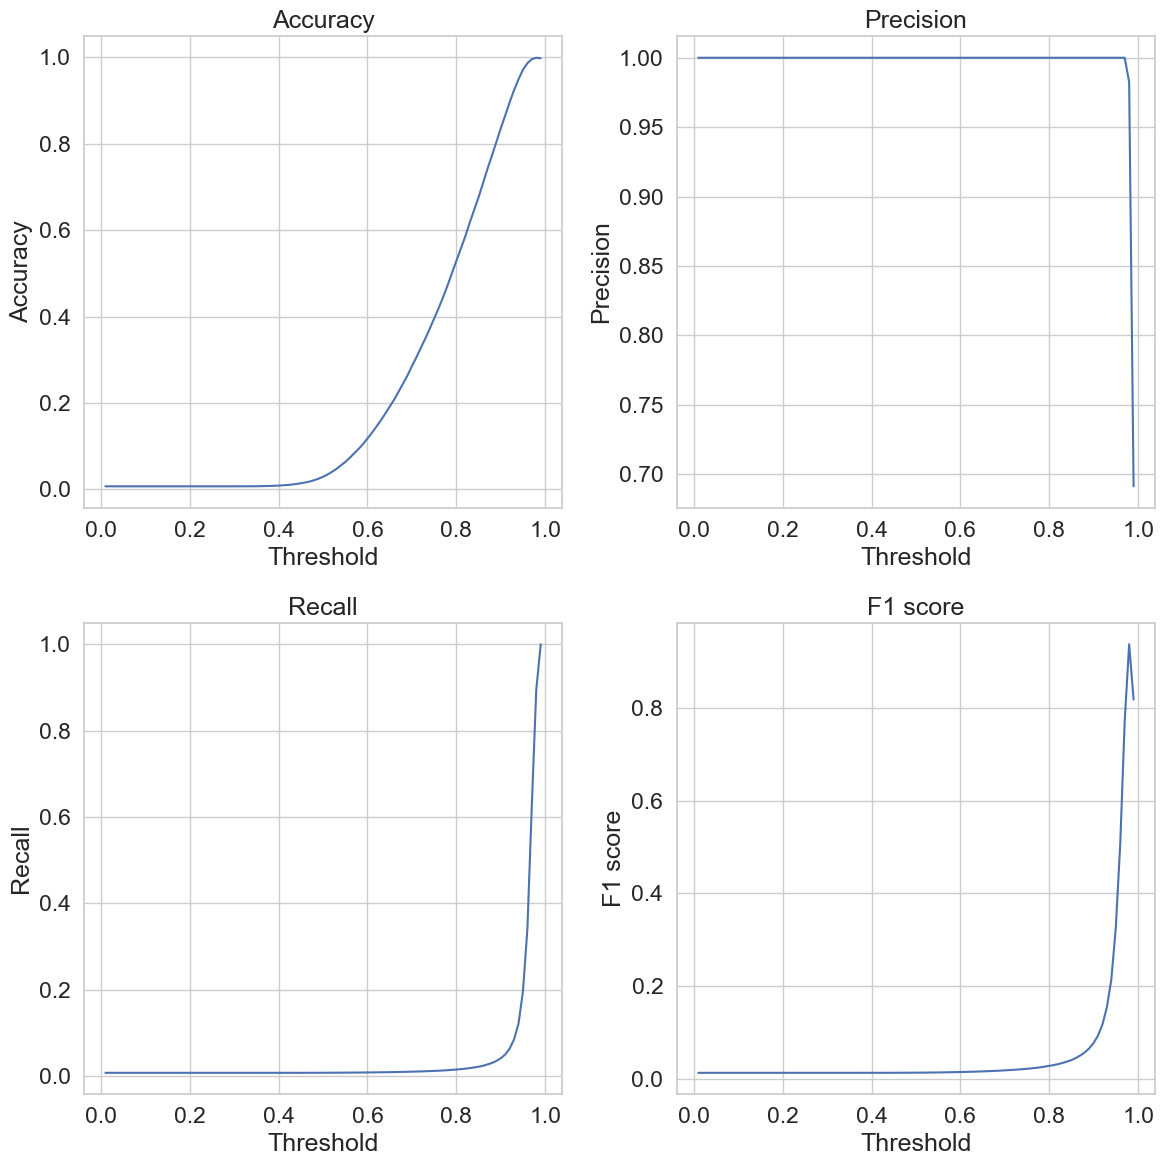
\includegraphics[width=0.9\linewidth]{img/img-metrics}
	\caption{Evaluation metrics as a function of the cosine similarity threshold. The plots show how accuracy, precision, recall, and F1 score evolve across thresholds ranging from 0 to 1. This analysis helps identify the optimal decision boundary that balances classification performance in the context of an imbalanced speaker verification dataset.}
	\label{fig:img-metrics}
\end{figure}

The confusion matrix components were computed for each threshold value in the range [0.01, 1.00]. True positives represent correctly identified same-speaker pairs, while true negatives correspond to correctly rejected different-speaker pairs. False positives occur when different-speaker pairs are incorrectly classified as same-speaker and false negatives represent missed detections of same-speaker pairs.

The results show, as expected, that at low thresholds, the model over-predicts same-speaker relationships, leading to high false positive and false negative counts. As the threshold increases, false positives decrease while false negatives increase. The true negative count rises steadily with the threshold, whereas true positives remain relatively flat due to the limited number of same-speaker comparisons.

Figure~\ref{fig:img-metrics} presents accuracy, precision, recall, and F1 score plotted as functions of the cosine similarity threshold. This analysis aims to identify the threshold that achieves the best trade-off between correctly identifying same-speaker pairs and avoiding false classifications.

The accuracy curve shows a steep rise beginning around threshold 0.85, eventually approaching 1.0. However, given the imbalance in the dataset, accuracy alone is not a reliable metric. Precision remains nearly constant and close to 1.0 across all thresholds until a sharp drop near 1.0, indicating that when the model does predict a pair as same-speaker, it is almost always correct, though such predictions are rare.

Recall values are close to zero across most thresholds and only increase sharply at the high end, suggesting that most same-speaker pairs are missed unless a very high threshold is applied. This behaviour is reflected in the F1 score, which stays low until it peaks abruptly at a threshold near 0.97–0.99, indicating a narrow window where precision and recall are reasonably balanced.

These curves reinforce the importance of using the F1 score in threshold selection for imbalanced data. The optimal threshold corresponds to the peak of the F1 score curve, where the model achieves its best-combined performance in identifying same-speaker pairs while maintaining high precision. The maximum F1, calculated from this plot, had a value of \texttt{0.93645} and occurred at threshold \texttt{0.98}.



\section{Analysis and discussion}

\section{Conclusion and future work}




\section*{Generative AI}

\printbibliography


	
\end{document}
